\chapter{Methodology}
\label{methodology}


\section{Overview}

This chapter describes the design, implementation, and deployment workflow of the SoH estimation framework at the center of this thesis. As established in Chapter~\ref{introduction}, the work operates within a dual-model Digital Twin architecture proposed by Alamin~\autocite{Alamin2023}: a SoH model tracks long-term battery degradation, while a SoC model, receiving the SoH estimate as input, can be updated over the air as the battery ages. This thesis focuses on the SoH foundation layer---building, compiling, deploying, and validating the degradation-tracking model---and on designing the OTA mechanism that would eventually serve the SoC model.

The workflow from raw battery data to a deployed SoH model consists of five stages, shown in Figure~\ref{fig:ch3_ml_workflow}.

\begin{figure}[H]
    \centering
    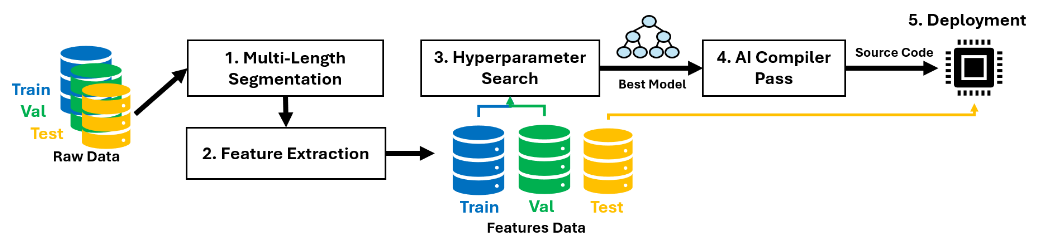
\includegraphics[width=1\linewidth]{images/ch3_ml_workflow.png}
    \caption{High-level overview of the training and deployment workflow: multi-length segmentation, feature extraction, hyperparameter search, AI compiler pass, and MCU deployment.}
    \label{fig:ch3_ml_workflow}
\end{figure}

The five stages are:

\begin{enumerate}
    \item \textbf{Data acquisition and preprocessing} (Section~\ref{sec:ch3_data}). Public NASA battery datasets are organized by discharge cycle, optionally normalized, and split into training, validation, and test sets.
    \item \textbf{Multi-length window segmentation} (Section~\ref{sec:ch3_segmentation}) and \textbf{feature extraction} (Section~\ref{sec:ch3_features}). Each discharge cycle is sliced into windows of five different lengths. From each window, a fixed ten-dimensional feature vector is extracted, decoupling the model's input dimension from the raw window length.
    \item \textbf{Model training and hyperparameter search} (Section~\ref{sec:ch3_training}). A LightGBM gradient-boosted tree ensemble is trained on the pooled multi-length features, with hyperparameters optimized through Bayesian search under deployment-aware size constraints.
    \item \textbf{Model compilation} (Section~\ref{sec:ch3_compilation}). The trained ensemble is converted to self-contained C code via the EDEN compiler, extended by collaborators to support LightGBM's tree format.
    \item \textbf{MCU deployment and performance verification} (Sections~\ref{sec:ch3_deployment}--\ref{sec:ch3_verification}). The generated C code and a hand-written feature extraction routine are integrated into firmware for the SPC58EC80E5 automotive microcontroller. Estimation accuracy, inference latency, and memory footprint are measured, and a BiLSTM baseline is reproduced on the same hardware.
\end{enumerate}

Section~\ref{sec:ch3_ota} then describes the design of the OTA update mechanism that would close the cloud-to-edge loop in the full Digital Twin architecture.

Figure~\ref{fig:project_architecture} situates the deployment within the broader system. Once the SoH model is running on the vehicle, it produces real-time estimates from sensor data (steps 1--2). Operational data are periodically uploaded to the cloud (step 3). When SoH degradation triggers a retraining condition, the cloud retrains the SoC model (step 4) and delivers the update over the air (step 5). This thesis implements steps 1--2 for the SoH model and designs steps 3--5.

\begin{figure}[H]
    \centering
    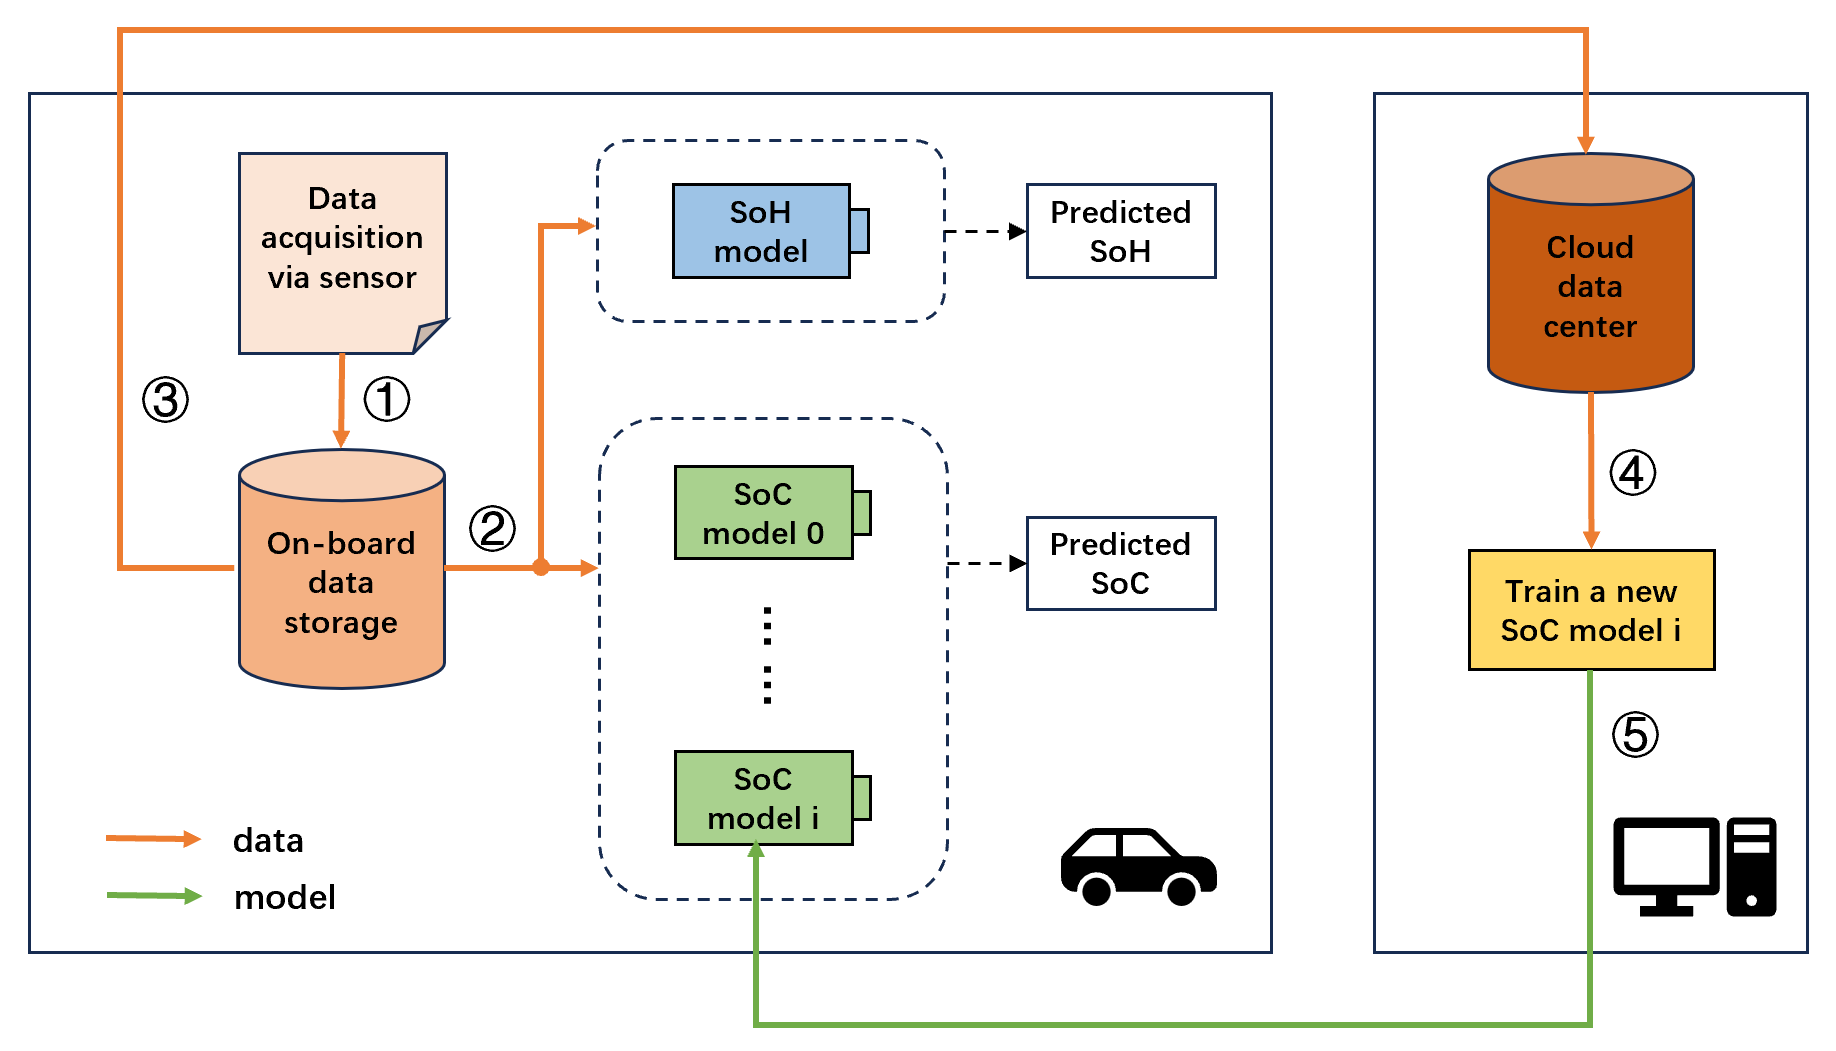
\includegraphics[width=1\linewidth]{images/ch3_project_architecture.png}
    \caption{Architecture of the proposed system: onboard SoH inference integrated with cloud-based model management and OTA delivery.}
    \label{fig:project_architecture}
\end{figure}


\section{Data Acquisition and Preprocessing}
\label{sec:ch3_data}

\subsection{Data Sources}

The work uses two public NASA lithium-ion battery datasets, summarized in Table~\ref{tab:dataset_source}. Both are widely cited in the SoH estimation literature, and they are the same datasets used by the BiLSTM baseline~\autocite{Sammartino2021}, ensuring a fair comparison. The two datasets differ in sampling rate, cell count, and usage patterns, which tests the model's ability to generalize.

\begin{table}[H]
    \centering
    \begin{adjustbox}{width={0.9\textwidth}, totalheight={\textheight}, keepaspectratio}
    \setcellgapes{3pt}
    \makegapedcells
    \begin{tabular}{c c c c}
    \hline
    Dataset & Battery Type & Sampling Rate & SoH Label \\
    \hline
    NASA Battery (NBD) \autocite{nasa_battery_2007} & 18650 Li-ion & 0.09\,Hz & Capacity per cycle \\
    \makecell{Randomized Battery Usage \\ (NRD) \autocite{nasa_data_randomized}} & 18650 LCO (28 cells) & 0.33\,Hz & SoH per cycle \\
    \hline
    \end{tabular}
    \end{adjustbox}
    \caption{Datasets used in this work}
    \label{tab:dataset_source}
\end{table}

Each dataset consists of charge/discharge experiment logs. Each file contains rows of measurements (voltage $V$, current $I$, temperature $T$, relative timestamp $t$) collected during successive discharge cycles. Every row in a cycle shares the same SoH label---the measured discharge capacity for that cycle. Figure~\ref{fig:ch3_inputdata_sample} shows the raw data structure.

\begin{figure}[H]
    \centering
    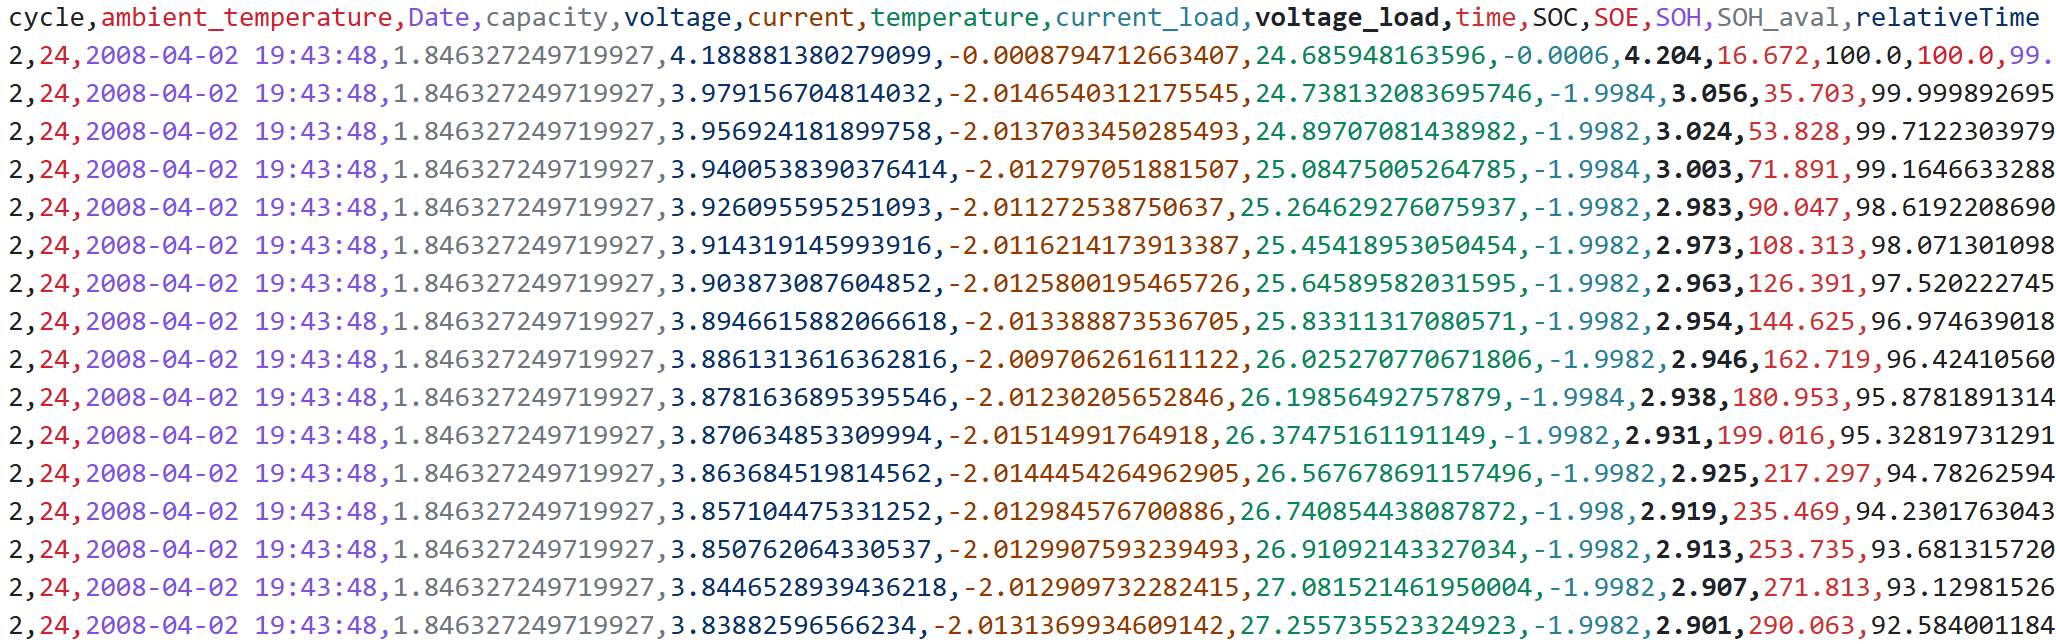
\includegraphics[width=0.5\linewidth]{images/ch3_inputdata_sample.png}
    \caption{Structure of the raw input data: rows correspond to sampling instants within discharge cycles; all rows in a cycle share the same SoH label.}
    \label{fig:ch3_inputdata_sample}
\end{figure}

\subsection{Preprocessing}

Preprocessing consists of two steps. First, the raw data are grouped by discharge cycle, so that each cycle forms an independent unit. Second, an optional MinMax scaling step maps the continuous variables ($V$, $I$, $T$) to $[0, 1]$. For tree-based models like LightGBM, scaling is not strictly required---splits depend only on feature ordering, not on absolute magnitudes. It is applied here to keep experimental conditions uniform across models (the BiLSTM baseline benefits from normalized inputs). No filtering or outlier removal was performed; the NASA datasets are used as distributed.

\subsection{Train/Validation/Test Split}

Data are partitioned at the cycle level, not at the individual sample level. This is important: if rows from the same discharge cycle appeared in both training and test sets, the model could exploit within-cycle autocorrelation rather than learning genuine degradation patterns, inflating accuracy estimates.

The split proceeds in two stages. First, 80\% of the discharge cycles are assigned to a combined training-plus-validation pool and 20\% to the test set. Second, the training-plus-validation pool is randomly partitioned into 80\% training and 20\% validation cycles. The resulting overall proportions are 64\% training, 16\% validation, and 20\% test. The same two-stage split is applied to both NBD and NRD.

For the NRD dataset, which contains 28 cells, an additional constraint is enforced: all cycles from a given cell go to the same partition. The test set contains cells the model never saw during training or validation. This evaluates cross-cell generalization---a stricter and more realistic test than evaluating on unseen cycles from known cells.


\section{Multi-Length Window Segmentation}
\label{sec:ch3_segmentation}

\subsection{Motivation}

Most published SoH models, including the BiLSTM baseline~\autocite{Sammartino2021}, operate on fixed-length input windows. The BiLSTM was trained with 20-sample windows; it cannot process a 40-sample or 60-sample window without architectural changes. In the field, however, the effective window duration varies: the BMS sampling rate may differ across hardware revisions, and discharge events can be arbitrarily short (a brief trip) or long (a highway drive). A model tied to one window length becomes a maintenance liability.

The approach taken here is straightforward: instead of training on a single window length, we train on several at once. If the model sees features computed from windows of many different lengths during training, it learns that window length itself should not affect the SoH estimate. After deployment, the model remains accurate under a range of operating conditions without retraining.

\subsection{Method}

For each discharge cycle (a sequence of $n$ samples), sliding windows are extracted for every window length $wlen \in \{20, 30, 40, 50, 60\}$ with a stride equal to the window length (no overlap):

\begin{verbatim}
for wlen in [20, 30, 40, 50, 60]:
    step = wlen
    for i in range(0, n - wlen + 1, step):
        x_win = data[i : i + wlen]
        y_win = label[i + wlen - 1]
\end{verbatim}

A cycle with $n = 210$ samples produces 10 windows at $wlen = 20$, 7 windows at $wlen = 30$, and so on. The five lengths were chosen because they span the range commonly used in the SoH literature and together cover short windows (capturing local dynamics) to longer windows (capturing trend information).

Figure~\ref{fig:ch3_window_segementation} illustrates the process: a single discharge sequence is sliced into multiple groups of windows, one group per window length. Each window becomes an independent training sample.

\begin{figure}[H]
    \centering
    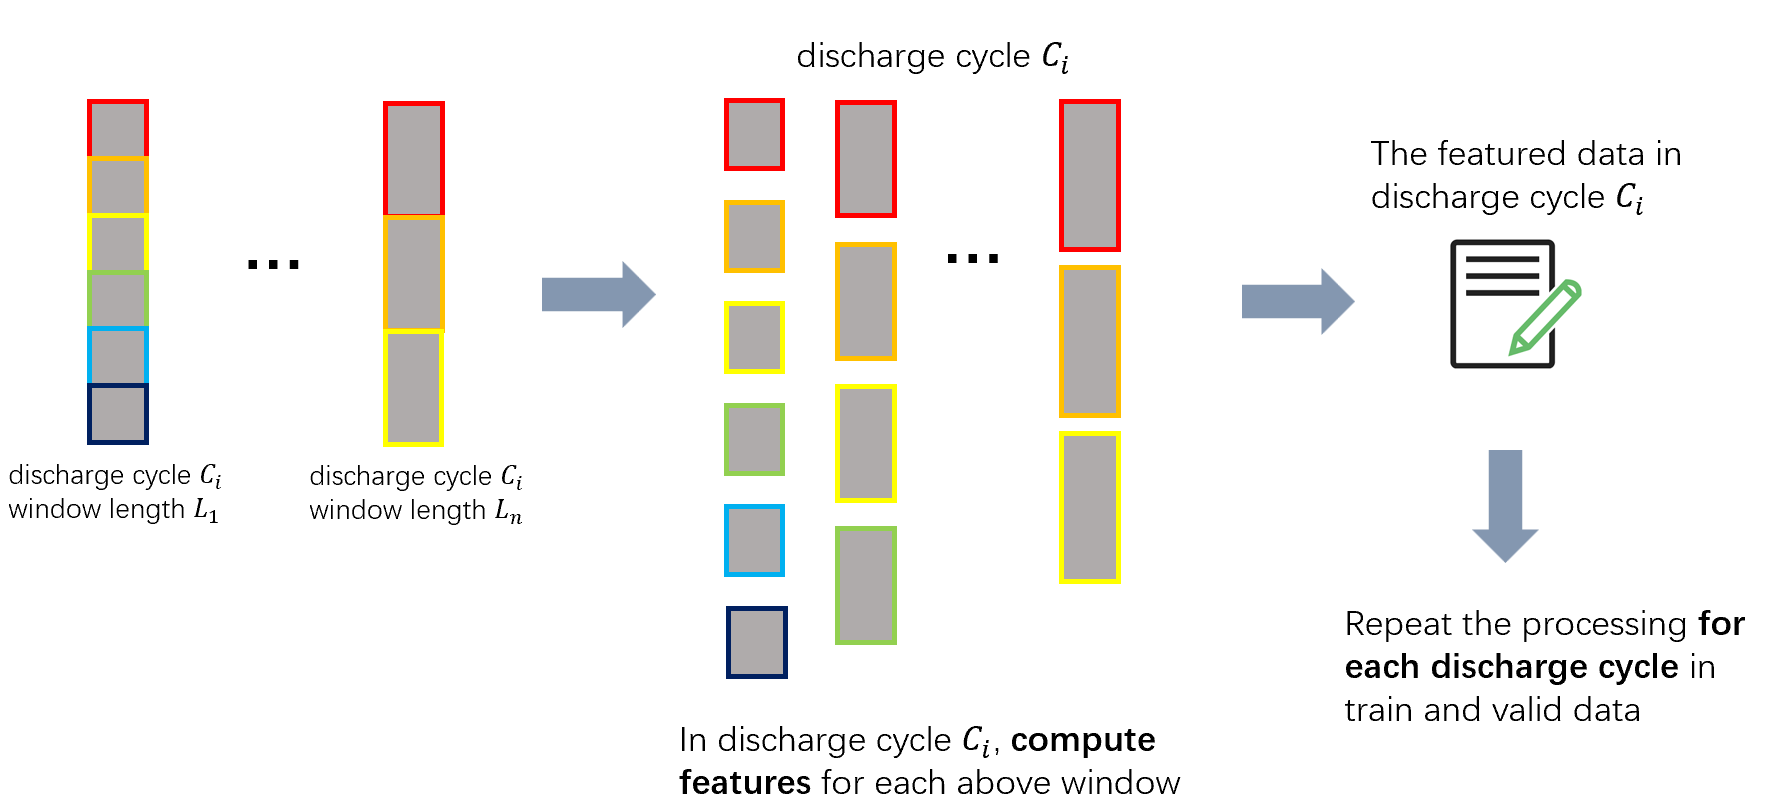
\includegraphics[width=1\linewidth]{images/ch3_window_segementation.png}
    \caption{Multi-length segmentation: each discharge cycle is sliced into windows of five different lengths, producing training samples at multiple temporal resolutions.}
    \label{fig:ch3_window_segementation}
\end{figure}

\subsection{Label Assignment}

The label for each window is taken from the last row of that window (\texttt{label[i + wlen - 1]}). This convention was originally designed for SoC estimation, where the label (SoC) changes at each time step and the last value in the window is the most recent. For SoH, the label is constant across the entire cycle, so taking the last row is equivalent to taking any row. The implementation detail is noted here because it reflects the dual-model origin of the codebase: the same segmentation routine serves both SoH and SoC tasks.

\subsection{Data Augmentation Effect}

Because each cycle is sliced at five different window lengths, the training set contains roughly five times as many samples as a single-length segmentation would produce. The model sees the same physical discharge event at multiple temporal resolutions. The training objective becomes: \emph{regardless of window length, predict the same SoH}. This inductive bias is what makes the deployed model robust to varying input conditions.


\section{Feature Extraction}
\label{sec:ch3_features}

\subsection{Design Rationale}

A window of raw data is a matrix of $wlen \times 4$ values ($V$, $I$, $T$, $t$). This cannot be fed directly to LightGBM, which expects a fixed-size input vector. The role of feature extraction is to compress the variable-length sequence into a fixed-length numerical description that preserves the information relevant to SoH estimation.

The feature set, inspired by Alamin et al.~\autocite{feature_eng}, captures the statistical behavior of the battery during the discharge window. Rather than modeling every sample, we summarize the window through trends and aggregates---quantities that a battery engineer would examine when assessing degradation: how fast the voltage drops, how much the temperature rises, and how the voltage--capacity relationship shifts.

\subsection{Intermediate Quantities}

Before extracting the final features, five intermediate signals are computed from the raw samples within each window:

\begin{table}[H]
    \centering
    \setcellgapes{3pt}
    \makegapedcells
    \begin{tabular}{c c c}
    \hline
    Signal & Symbol & Formula \\
    \hline
    Voltage change rate & $\dot{V}$ & $dV/dt$ \\
    Temperature change rate & $\dot{T}$ & $dT/dt$ \\
    Power & $P$ & $V \times I$ \\
    Cumulative capacity & $Q$ & $\int_{t_0}^{t} I(\tau)\, d\tau$ \\
    Voltage derivative w.r.t.\ capacity & $dV/dQ$ & $(dV/dt)\,/\,(dQ/dt)$ \\
    \hline
    \end{tabular}
    \caption{Intermediate signals computed within each window}
    \label{tab:intermediate_signals}
\end{table}

Among these, $dV/dQ$ carries particular diagnostic value. In the battery literature, incremental capacity (IC) analysis uses the positions and heights of peaks in $dQ/dV$ (the reciprocal of $dV/dQ$) to identify degradation modes such as loss of active material and loss of lithium inventory. As the battery ages, these peaks shift in position and shrink in amplitude. Capturing the range of $dV/dQ$ within a window---its mean, maximum, and minimum---encodes these aging-induced changes.

\subsection{Final Ten-Dimensional Feature Vector}

The intermediate signals are summarized through averaging (and, for $dV/dQ$, through min/max) over the window. This yields a ten-dimensional feature vector:

\begin{enumerate}
    \item Mean discharge voltage rate --- $\text{mean}(dV/dt)$
    \item Mean voltage --- $\text{mean}(V)$
    \item Mean discharge temperature rate --- $\text{mean}(dT/dt)$
    \item Mean power --- $\text{mean}(V \times I)$
    \item Mean relative timestamp --- $\text{mean}(t_{rel})$
    \item Mean $dV/dQ$
    \item Maximum $dV/dQ$
    \item Minimum $dV/dQ$
    \item Window duration --- $t_{last} - t_{first}$
    \item Mean temperature --- $\text{mean}(T)$
\end{enumerate}

The key property of this feature vector is that its size is independent of the original window length. Whether the window contains 20 samples or 60, the output is always 10 numbers. This is the property that allows a single LightGBM model to process windows of arbitrary length.

\subsection{MCU Implementation}

The same feature extraction logic is implemented twice: in Python (NumPy/Pandas) for offline training, and in hand-written C for on-board execution. The C implementation receives a raw data buffer ($V$, $I$, $T$, $t$ arrays of length $wlen$), computes the five intermediate signals sample by sample, then reduces them to the ten statistical features. All arithmetic uses single-precision floating point. The SPC58EC80E5 includes a hardware FPU, so these operations execute at native speed with no software emulation overhead. The full C source is reproduced in Appendix~\ref{app:feature_extraction}.


\section{Model Training and Hyperparameter Search}
\label{sec:ch3_training}

\subsection{Choice of LightGBM}

The rationale for choosing LightGBM was laid out in Chapter~\ref{background} (Section~\ref{sec:bg_soh_methods}). In brief: tree ensembles offer competitive regression accuracy, inference consists entirely of threshold comparisons and additions (no matrix multiplies, no activation functions), the model takes a fixed-size feature vector regardless of the original window length, and the ensemble can be compiled to self-contained C code with zero external dependencies. These properties align directly with the requirements of automotive MCU deployment.

\subsection{Bayesian Hyperparameter Search}

LightGBM exposes several hyperparameters that govern model capacity, regularization, and training dynamics. Finding a configuration that balances estimation accuracy against model size (which determines Flash footprint) is non-trivial. A Bayesian search using Optuna (v4.2.0) with the TPE (Tree-structured Parzen Estimator) sampler explores the space efficiently. The search objective is minimization of MAE on the validation set. A total of 1{,}000 trials are run. Each trial trains to completion (the number of trees specified by \texttt{n\_estimators}); no early-stopping patience is applied.

Table~\ref{tab:hp_space} lists the search space. Two parameters are constrained by deployment requirements: \texttt{max\_depth} is capped at 8 and \texttt{num\_leaves} at 25. These caps prevent the search from producing models too large to fit in the MCU's Flash. A tree ensemble's Flash footprint scales as $O(N_{trees} \times 2^{depth})$. At depth 8, a single fully-grown tree contains at most $2^8 - 1 = 255$ nodes; with 400 trees, even the worst-case total (approximately 100{,}000 nodes, or 800\,KB) fits comfortably within the SPC58's 4\,MB Flash.

\begin{table}[H]
    \centering
    \setcellgapes{3pt}
    \makegapedcells
    \begin{tabular}{c c}
    \hline
    Parameter & Search Range \\
    \hline
    Learning Rate & $[10^{-5}, 10^{-1}]$ \\
    Max Depth & $[3, 8]$ \\
    Num Leaves & $[2, 25]$ \\
    Num Estimators & $[50, 450]$ \\
    $\alpha$ (L1 regularization) & $[10^{-6}, 1]$ \\
    $\beta$ (L2 regularization) & $[10^{-6}, 1]$ \\
    Min Child Samples & $[2, 25]$ \\
    Column Samples by Tree & $[0.1, 1]$ \\
    \hline
    \end{tabular}
    \caption{Hyperparameter search space}
    \label{tab:hp_space}
\end{table}

\subsection{Training Procedure}

Features extracted from all five window lengths are pooled into a single training set. Each sample is a 10-dimensional feature vector with its SoH label. Validation uses the same mixed-length scheme: the model is evaluated on validation samples drawn from all window lengths, ensuring the selected hyperparameters perform well across the board.

The best trial (lowest validation MAE) yields the final model. The hyperparameter values and the corresponding accuracy figures are reported in Chapter~\ref{experiment}. The training infrastructure is built on LightGBM 4.5.0; a complete list of Python dependencies and their versions appears in Appendix~\ref{app:dependencies}.

% GitHub repository footnote
The code for data preprocessing, feature extraction, model training, and evaluation is available at \url{https://github.com/...}.\footnote{Repository URL to be added.}

\subsection{Contrast with Deep Learning}

A practical difference between LightGBM and the BiLSTM baseline is worth highlighting. Because a BiLSTM's input dimension is fixed at training time, covering five window lengths requires training five separate BiLSTM models. LightGBM requires one---the same ensemble handles all window lengths because the feature vector size does not change. At deployment time, the Flash holds a single model, regardless of the BMS sampling configuration.


\section{Model Compilation: EDEN to C}
\label{sec:ch3_compilation}

\subsection{From Python to MCU}

A trained LightGBM model is a Python Booster object. To run on the MCU, it must be translated into C code that is self-contained (no external libraries), statically allocated (no \texttt{malloc}), recursion-free (bounded stack depth), and compilable with a bare-metal cross-compiler.

EDEN (Efficient Decision tree Ensembles) is an open-source compiler originally developed for deploying random forests on IoT edge nodes~\autocite{Eden}. For this thesis, EDEN was extended by collaborators to support LightGBM's gradient-boosted tree format. The author used the extended compiler to convert trained LightGBM models into C.

[TODO: EDEN compilation flow diagram --- to be provided]

\subsection{In-Memory Tree Representation}

EDEN serializes each decision tree in the ensemble into four static arrays:

\begin{itemize}
    \item \textbf{Split threshold / leaf value array} (\texttt{float32}). For internal nodes: the feature threshold against which the input is compared. For leaf nodes: the tree's output contribution (not the final SoH prediction, but the additive term for this tree).
    \item \textbf{Feature index array} (\texttt{uint16}). For internal nodes: the index (0--9) of the input feature used for the split. For leaf nodes: set to \texttt{\#Features} (10), serving as a leaf marker.
    \item \textbf{Right child index array} (\texttt{uint16}). Nodes are laid out in pre-order, so the left child of node $k$ is implicitly at index $k+1$. Only the right child's index needs to be stored explicitly. For leaf nodes this field is unused.
    \item \textbf{Root index array} (\texttt{uint16}). The starting position of each tree in the node arrays, enabling iteration over all trees in a simple loop.
\end{itemize}

\subsection{Inference Procedure}

Inference on an input feature vector \texttt{x[0..9]} proceeds as follows:

\begin{verbatim}
prediction = 0.0
for each tree t:
    idx = root_index[t]
    while feature_index[idx] <= 9:       // not a leaf
        if x[feature_index[idx]] <= threshold[idx]:
            idx = idx + 1                // left child = next position
        else:
            idx = right_child[idx]       // right child = explicit index
    prediction += threshold[idx]         // leaf value = tree output
return prediction
\end{verbatim}

No function calls, no recursion, no dynamic allocation. On the SPC58, the outer loop and inner tree traversal compile into compact sequences of load-compare-branch instructions.

\subsection{Model Size}

The four arrays are declared \texttt{const} and placed in Flash. The exact Flash footprint depends on the number of trees and their actual depth (trees rarely grow to the maximum allowed depth). For the configurations used in this work, the model occupies [TODO: insert exact KB values] of the SPC58's 4\,MB Flash (under 3\%, as reported in Chapter~\ref{experiment}). The generated code consists of one \texttt{.c} file (array definitions and the inference function) and one \texttt{.h} file (function declaration). Both are added directly to the SPC5Studio project.


\section{MCU Deployment}
\label{sec:ch3_deployment}

\subsection{Target Hardware}

The deployment target is the SPC58EC80E5, an automotive-grade microcontroller by STMicroelectronics. Key specifications: dual-core Power Architecture e200z420n3 at 120\,MHz, 4\,MB on-chip Flash, 608\,KB on-chip SRAM, ISO~26262 ASIL-B support, and a full set of automotive communication peripherals (CAN FD, LIN, Ethernet). The device is part of ST's BMS evaluation kit, which also includes an electrical isolation unit and a battery analog front-end. The author assembled the full kit; the deployment described here uses the SPC58 board alone, feeding pre-recorded test data over a serial connection. This isolates the inference workload from the physical variables of the analog front-end and battery cells.

\subsection{Toolchain}

Two software tools are used. \textbf{SPC5Studio IDE} (Eclipse-based) provides the GCC Power Architecture cross-compiler, the SPC5 Hardware Abstraction Layer (HAL), and the Flash programming utility. Compilation uses \texttt{-O2} optimization. \textbf{UDE Starterkit} (Universal Debug Engine, PLS) provides run-control debugging: breakpoints, single-stepping, memory inspection, and cycle-count measurement.

[TODO: firmware architecture block diagram --- to be provided]

\subsection{Firmware Integration}

The SPC58 firmware integrates the following components:

\begin{enumerate}
    \item \textbf{HAL initialization} (auto-generated by SPC5Studio): clock tree, GPIO, and serial port setup.
    \item \textbf{Feature extraction module} (hand-written C): receives a window of raw data ($V$, $I$, $T$, $t$ arrays), computes the ten features, and returns a \texttt{float[10]}.
    \item \textbf{Model inference module} (EDEN-generated C): receives the feature vector, traverses all trees, and returns the SoH prediction.
    \item \textbf{Main loop}: reads a data window from the serial input, calls feature extraction and inference in sequence, and transmits the result back over serial.
\end{enumerate}

All data---model arrays, feature extraction buffers, serial buffers---are statically allocated at compile time. The stack depth is bounded: tree traversal uses a \texttt{while} loop rather than recursion.

\subsection{Test Procedure}

Deployment validation has two aspects:

\textbf{Functional correctness.} A small set of real discharge windows is run through the MCU, and the inference output is compared bit-for-bit against the Python model's output on the same data. The two match, confirming that the C implementation is logically equivalent to the Python reference. This check is performed once during initial deployment and not repeated.

\textbf{Performance measurement.} CPU cycle counts are measured by running the inference pipeline on randomly generated window data (the cycle count depends on window length and model structure, not on the specific numerical values of the data). The UDE cycle counter reports the number of clock cycles from feature extraction start to inference completion. Multiple runs yield variations below 1\%, so single measurements are reported directly. Flash and RAM usage are read from the SPC5Studio linker map file.

\textbf{Accuracy evaluation.} MAE and MSE are evaluated in the Python training environment on the held-out test set, rather than by running every test window through the MCU. Since the MCU output has been verified to match the Python output, MCU-based accuracy evaluation would produce identical numbers at far greater effort.


\section{Performance Verification}
\label{sec:ch3_verification}

The deployed system is evaluated along four dimensions. The metrics themselves are defined here; the results appear in Chapter~\ref{experiment}.

\subsection{Estimation Accuracy}

Two error metrics are computed on the test set:

\begin{equation}
\text{MAE} = \frac{1}{N} \sum_{i=1}^{N} |\hat{y}_i - y_i|
\end{equation}
\begin{equation}
\text{MSE} = \frac{1}{N} \sum_{i=1}^{N} (\hat{y}_i - y_i)^2
\end{equation}

where $\hat{y}_i$ is the predicted SoH, $y_i$ is the ground truth, and $N$ is the number of test samples. MAE has the same unit as the label (capacity in Ah for NBD, percentage for NRD) and is the primary metric. MSE penalizes large errors more heavily and is reported as a secondary indicator.

Accuracy is reported for two subsets of the test data:

\begin{itemize}
    \item \textbf{FW (First Window):} only the first window of each discharge cycle. This follows the protocol of Sammartino et al.~\autocite{Sammartino2021}: the model should produce an accurate SoH estimate from the earliest available data in a cycle. For comparison with the BiLSTM baseline (which was trained for $wlen = 20$), FW results are reported at $wlen = 20$.
    \item \textbf{Full:} all windows in the test set, reflecting performance at any point during a discharge event.
\end{itemize}

\subsection{Inference Efficiency}

The CPU cycle count for one complete inference (feature extraction plus model traversal) is measured via the UDE cycle counter. The corresponding wall-clock latency is $t_{inf} = cycles / 120\,\text{MHz}$. The BiLSTM baseline is measured under identical conditions.

\subsection{Memory Footprint}

Flash usage (model arrays, firmware code, HAL, feature extraction) and RAM usage (feature buffers, stack, HAL globals) are extracted from the SPC5Studio linker map. Values are reported in absolute bytes and as percentages of the available 4\,MB Flash and 608\,KB SRAM.

\subsection{Generalization to Unseen Window Lengths}

The model is trained on $wlen \in \{20, 30, 40, 50, 60\}$. To test robustness, MAE is also evaluated on window lengths not seen during training: $wlen \in \{10, 35, 55, 75\}$. These test lengths are chosen to fall both inside and outside the training range. A single LightGBM model is evaluated on all test lengths without modification---the feature extraction pipeline handles any window length natively.

For the BiLSTM baseline, which cannot process variable-length inputs, unseen window lengths are accommodated through heuristic adaptation---trimming the oldest samples for longer windows, and zero-padding for shorter ones---to provide a reference comparison. [TODO: confirm BiLSTM adaptation strategy after code review]


\section{OTA Update Architecture Design}
\label{sec:ch3_ota}

The preceding sections describe a complete pipeline for training, compiling, and deploying a SoH model. Once deployed, however, the model must remain accurate over years of battery aging. This section designs the OTA mechanism that would eventually keep the SoC model current within the Digital Twin architecture. To be clear: the OTA mechanism described here is an architectural design; it has not been implemented in hardware.

\subsection{Role in the Architecture}

The SoH model itself is designed for deployment-time robustness (multi-length training, see Section~\ref{sec:ch3_segmentation}) and does not require frequent updates. The SoC model, in contrast, depends on the current SoH estimate as an input. When the battery's SoH has drifted by a meaningful amount since the last SoC model update, the old model's parameters no longer match the battery's current characteristics. OTA provides the channel to refresh the SoC model without physical access to the vehicle.

\subsection{Update Triggers}
\label{sec:ch3_ota_triggers}

Two conditions trigger a cloud-side SoC model retraining:

\begin{enumerate}
    \item \textbf{SoH drift.} The vehicle periodically uploads operational data to the cloud. When the current SoH estimate differs from the baseline recorded at the last SoC update by more than a predetermined threshold (e.g., 1 percentage point), retraining is triggered. The rationale: enough degradation has accumulated that the battery's discharge characteristics have measurably changed.
    \item \textbf{Timeout.} If more than a preset interval (e.g., six months) has elapsed since the last update, retraining is triggered regardless of drift. This acts as a safety net against gradual, sub-threshold accuracy erosion.
\end{enumerate}

Both triggers are designed to keep update frequency low (on the order of months), minimizing the communication and validation burden.

\subsection{Update Workflow}

A complete OTA update cycle consists of eight steps:

\begin{enumerate}
    \item \textbf{On-board data accumulation.} During normal operation, the BMS buffers sensor data ($V$, $I$, $T$, and the SoH estimate) in on-board storage, organized in the same window format used for training.
    \item \textbf{Periodic upload.} When the buffer reaches a capacity threshold or a time interval elapses, the accumulated data are uploaded to the cloud via the vehicle's Telematics Control Unit (TCU). Upload occurs only when the vehicle is in a safe state (parked, sufficient battery, good network signal).
    \item \textbf{Retraining trigger evaluation.} The cloud checks the two trigger conditions (Section~\ref{sec:ch3_ota_triggers}) against the uploaded SoH estimates.
    \item \textbf{Model retraining.} If triggered, a new SoC model is trained on the cloud using data accumulated since the last update. The training pipeline mirrors the one described in this chapter, with SoC as the target variable.
    \item \textbf{Validation and packaging.} The retrained model is validated against a held-out subset of the new data. If accuracy improves measurably over the current model, the model parameters (the four EDEN arrays) are serialized, compressed, and digitally signed with the cloud's private key.
    \item \textbf{OTA delivery.} The vehicle is notified of the available update. The signed package is downloaded over the cellular connection when conditions permit. Integrity (SHA-256 hash) and authenticity (signature verification with the cloud's public key) are checked before installation proceeds.
    \item \textbf{A/B partition installation.} The update is written to the inactive Flash partition while the BMS continues operating from the active partition. After the write completes, a checksum of the inactive partition is verified.
    \item \textbf{Model switch and confirmation.} On the next BMS restart (or on a cloud command), the bootloader switches the active partition. The vehicle reports the update outcome (success, failure, or rollback) to the cloud for audit and trigger reset.
\end{enumerate}

\subsection{Security and Version Control}

The design incorporates standard automotive OTA security practices: digital signatures prevent tampering, monotonically increasing version numbers prevent rollback attacks, and hash verification catches transmission errors. The SPC58 platform supports hardware-assisted secure boot in production configurations, though the security features have not been tested as part of this thesis.

\subsection{Fallback and Recovery}

Model updates, unlike firmware updates, carry low risk: even a poorly trained model degrades SoC accuracy gradually, and the effect is reversible. The design includes three recovery mechanisms:

\begin{itemize}
    \item \textbf{A/B partition rollback.} If the new model produces anomalous outputs (SoC outside $[0, 100]\%$, rapid fluctuations inconsistent with battery physics, or persistent deviation from the Coulomb-counting estimate), the system atomically switches the active partition pointer back to the previous model.
    \item \textbf{Golden Model.} A factory-programmed conservative model, stored in a write-protected Flash region, serves as the last-resort fallback if both A and B partitions become corrupted. This model is burned at production time and is not modifiable over the air. (Note: the Golden Model is a design concept; no such image was programmed during this thesis.)
    \item \textbf{Cloud alerting.} Any rollback event is reported to the cloud, triggering an investigation of the problematic model and preventing its redistribution to other vehicles.
\end{itemize}

\subsection{Scope and Limitations}

The OTA design is presented at the architectural level. Communication protocol details (CAN frame formats, cellular transport), cloud infrastructure implementation, and end-to-end security testing are outside the scope of this thesis and represent directions for future work (Chapter~\ref{conclusion}).
